\documentclass[conference]{IEEEtran}
\IEEEoverridecommandlockouts

\usepackage[T1]{fontenc}
\usepackage{cite}
\usepackage{amsmath,amssymb,amsfonts}
\usepackage{graphicx}
\usepackage{booktabs}
\usepackage{multirow}
\usepackage{xcolor}
\usepackage{tikz}
\usetikzlibrary{positioning,arrows.meta,fit,backgrounds,calc,decorations.pathreplacing}
\usepackage[hidelinks]{hyperref}
\usepackage{url}

\newcommand{\verify}[1]{\textcolor{red}{[TODO: verify #1]}}
\newcommand{\Wtwo}{W_2}
\newcommand{\R}{\mathbb{R}}
\newcommand{\G}{\mathcal{G}}
\newcommand{\ci}[3]{\begin{tabular}[c]{@{}c@{}}$#1$\\[-1pt]{\scriptsize$[#2,\,#3]$}\end{tabular}}
\DeclareMathOperator*{\argmin}{arg\,min}
\DeclareMathOperator*{\argmax}{arg\,max}

\definecolor{cbull}{HTML}{009E73}
\definecolor{cbear}{HTML}{E69F00}
\definecolor{ccalm}{HTML}{56B4E9}
\definecolor{ccrisis}{HTML}{D55E00}
\definecolor{cblue}{HTML}{0072B2}

\begin{document}

\title{Causal Regime-Conditioned Trading Agent:\\ Verifiable Regime-Aware Reinforcement Learning}

\author{
\IEEEauthorblockN{Varad Durge, Ishaan Kawathekar, Tejas Putta}
\IEEEauthorblockA{\textit{Dept. of Electronics \& Computer Engineering}\\
\textit{SCTR's Pune Institute of Computer Technology}\\
Pune, India\\
varaddurge@gmail.com \verify{co-author e-mails}}
\and
\IEEEauthorblockN{Dr. Anjali A. Yadav}
\IEEEauthorblockA{\textit{Dept. of Electronics \& Computer Engineering}\\
\textit{SCTR's Pune Institute of Computer Technology}\\
Pune, India\\
\verify{guide e-mail and author order}}
}

\maketitle

\begin{abstract}
Regime-aware reinforcement-learning (RL) trading agents are usually judged by back-tested returns, which cannot show whether the regime signal actually drives their decisions. We present a reproducible pipeline that couples a Wasserstein regime-identity tracker with a suite of interventional tests on the trained policy. A four-state Gaussian hidden Markov model (HMM) is refitted every 42 four-hour bars on past rows only. Each new component is matched to persistent bull, bear, calm and crisis templates by the closed-form 2-Wasserstein distance, so regime names survive refits instead of being re-sorted. Two proximal policy optimisation (PPO) agents, identical except for four regime-probability inputs, are trained walk-forward on BTC/USDT data from 2021 to 2026. Every out-of-fold decision is audited by input ablation, counterfactual regime injection and a crisis-probability sweep. On 11{,}430 test bars, the tracker lowers the mean template-matching cost by a factor of 4.9 and gives labels whose volatility ordering is stable, but its non-injective matching starves the bull template, which is never issued after burn-in. The conditioned agent clearly uses its regime input: ablation moves its position on 60.7\% of bars, and it de-risks in bear and crisis segments. Yet only 0.1\% of bars pass all three checks, against 33.5\% for an archived run with moment-sorted labels. Reference policies confirm that the suite separates a faithful rule (97.9\%) from ignoring and inverted rules (0\%). The agent's Sharpe ratio of $-0.16$ (95\% CI $[-0.98, 0.63]$) beats its blind twin ($-1.12$) but not buy-and-hold ($0.35$). Faithfulness must therefore be re-verified whenever the regime layer changes.
\end{abstract}

\begin{IEEEkeywords}
regime detection, hidden Markov model, Wasserstein distance, optimal transport, reinforcement learning, algorithmic trading, explainability, faithfulness, counterfactual testing
\end{IEEEkeywords}

%======================================================================
\section{Introduction}
%======================================================================
Cryptocurrency markets move through very different conditions within a few years. Bitcoin rose sharply in 2021, lost roughly three quarters of its value between late 2021 and late 2022, and then spent 2023--2026 alternating between recoveries and drawdowns. A trading policy fitted to such a history without any notion of market state tends to learn one averaged behaviour that suits none of these phases. A natural remedy is to detect the prevailing regime and hand it to the policy as an extra input. Ndoutoumou \emph{et al.} combine a hidden Markov model with reinforcement-learning portfolio agents and report stronger risk-adjusted returns than the same agents without the regime signal~\cite{ndoutoumou2025hmm}. RegimeFolio builds sector portfolios around detected regimes in non-stationary markets~\cite{zhang2025regimefolio}, and explainable classifiers have been used to allocate assets by market state~\cite{zhang2020regimealloc}.

What this work rarely checks is whether the regime input matters. A regime-conditioned agent can report that it ``cut exposure because a crisis was detected'' while its actual computation ignores the crisis probability, or responds to it in the wrong direction. An explanation that is easy to understand is not necessarily faithful to the computation that produced the decision~\cite{mamalakis2025enigma}. Reviews of explainable machine learning find that explanations are often judged by whether users trust them, while standard tests of whether an explanation is true of the model are still missing~\cite{wiratsin2025xai}. Finance relies on much the same post-hoc tools, and their evaluation is uneven~\cite{yeo2025financial}. In high-stakes settings, the duty to explain a decision is not optional~\cite{reinhardt2025xai}.

A second, quieter problem sits inside the regime detector. An HMM refitted on new data returns its states in an arbitrary order, so ``state~2'' may mean crisis in one window and calm in the next. Sorting states by their moments after every fit repairs the names locally, but it forces four names onto whatever four components the latest fit produces, even if one of them no longer resembles anything seen before. We instead keep persistent bull, bear, calm and crisis templates and match each new component to the nearest template by the closed-form 2-Wasserstein distance, so a name survives a refit only when the component still resembles it.

This paper asks two linked questions. Does Wasserstein tracking give regime labels that keep their meaning across walk-forward refits? And when an RL agent is conditioned on those labels, does its behaviour depend on them in the way the labels' names imply? We answer both with a controlled experiment on BTC/USDT four-hour bars. Our contributions are:
\begin{itemize}
  \item A walk-forward implementation of Wasserstein template tracking for a four-state Gaussian HMM, with the closed-form diagonal $\Wtwo$ distance, probability aggregation and template smoothing written out as equations that match the released code.
  \item A per-decision verification suite of three interventions on the regime input (ablation, counterfactual injection and a sensitivity sweep), validated on reference policies that are faithful, regime-ignoring and inverted by construction.
  \item A twin experiment in which regime-conditioned and regime-blind PPO agents share architecture, seed and training budget, evaluated walk-forward with bootstrapped confidence intervals and a per-regime breakdown.
  \item An empirical finding: replacing moment sorting with Wasserstein tracking leaves the regime input load-bearing but collapses the faithfulness rate from 33.5\% to 0.1\%. We trace this to template starvation and to counterfactual inputs that lie outside the training distribution.
\end{itemize}

%======================================================================
\section{Related Work}
%======================================================================
\subsection{Regime detection}
Ndoutoumou, Yin and Cheng fit a Gaussian HMM and pass the inferred regime into reinforcement-learning agents on a Dow Jones portfolio. For several algorithms the hybrid agent improves the Sharpe and Sortino ratios relative to the same agent without the HMM~\cite{ndoutoumou2025hmm}. The comparison is on back-tested returns. It does not test whether the learned policy actually depends on the regime input. Tsang and Chen detect regime change in the foreign-exchange market with directional-change indicators, and use the detector to chart the period around Brexit~\cite{tsang2018regime}. Zhang, Yi and Chen use explainable machine learning to classify regimes and to support asset allocation~\cite{zhang2020regimealloc}. RegimeFolio is a regime-aware learning system for sectoral portfolio optimisation when markets are non-stationary~\cite{zhang2025regimefolio}. Standard HMMs switch state too readily on noisy data; we suppress this with a simple minimum-dwell rule, and we keep regime names stable across refits by Wasserstein template matching, described in Section~\ref{sec:method}.

\subsection{Reinforcement learning for portfolio optimisation}
Deep reinforcement learning is now a standard way to treat portfolio choice as a sequential decision. Surveys cover the single-agent literature and the move toward multi-agent systems~\cite{mortaji2024review,rout2026review}. Wang, Jin and Li cast asset-weight management as a Markov decision process and train a deep RL agent for diversification~\cite{wang2022drl}. Tamuly, Bhutani and Sukriti apply deep RL to dynamic capital allocation~\cite{tamuly2024drl}. Naik \emph{et al.} use proximal policy optimisation and deep deterministic policy gradient for real-time rebalancing on Indian equities, with the Sharpe ratio as the risk-adjusted objective~\cite{naik2025realtime}. Huang and Jing adapt a single-stock portfolio with a deep deterministic policy gradient agent~\cite{huang2025singlestock}. Gao and Tang evaluate advantage actor-critic and proximal policy optimisation on A-share portfolios drawn from CSI~300 constituents, under A-share trading constraints~\cite{gao2025drl}. Shrirao \emph{et al.} train portfolio policies intended to remain usable under adversarial market conditions~\cite{shrirao2025adversarial}. Across this work, a higher Sharpe ratio is treated as evidence that the agent has adapted. None of it checks whether a named regime input is what the policy uses.

\subsection{Explainability}
Mamalakis \emph{et al.} separate an explanation that is faithful to a deep network from one that is merely comprehensible~\cite{mamalakis2025enigma}. Wiratsin and Ragkhitwetsagul review whether explainable-AI techniques improve human trust, and they note the lack of standard evaluation metrics~\cite{wiratsin2025xai}. Reinhardt and Buchholz argue that explainability in high-stakes domains is an obligation, not only a convenience~\cite{reinhardt2025xai}. Yeo \emph{et al.} survey how post-hoc explanations are used in finance and how their limits affect decisions~\cite{yeo2025financial}. Our tests are different in kind: they intervene on one named input of a sequential policy rather than attributing a static prediction.

\subsection{Causal inference in financial decisions}
Qiu \emph{et al.} build a causal-inference model for stock-trend forecasting, on the view that predictive accuracy alone does not identify which dependencies the forecast uses~\cite{qiu2025cistf}. Katamaneni \emph{et al.} study machine-learning causal inference for decisions that must be revised as the environment changes~\cite{katamaneni2025causal}. Both treat causality as a property of the market time series. The interventions in this paper are different. The policy is a known function, so setting its regime input to a chosen value measures the effect of that input on the action, not a causal effect in the market.

%======================================================================
\section{Preliminaries}
%======================================================================
\subsection{Gaussian hidden Markov model}
Let $x_t\in\R^3$ be the regime features at bar $t$. A $K$-state Gaussian HMM has latent states $z_t\in\{1,\dots,K\}$, a transition matrix $A_{ij}=P(z_{t+1}=j\mid z_t=i)$, initial probabilities $\pi_0$ and emissions $x_t\mid z_t=k\sim\mathcal N(m_k,\Sigma_k)$. We use diagonal $\Sigma_k=\mathrm{diag}(v_k)$. Parameters are fitted by expectation--maximisation. The posterior $\gamma_t(k)=P(z_t=k\mid x_{1:n})$ comes from the forward--backward recursion and the most likely path from Viterbi decoding. The likelihood is invariant to permuting the state indices, so two fits on overlapping data can return the same regimes under different indices.

\subsection{2-Wasserstein distance between Gaussians}
For probability measures $\mu,\nu$ on $\R^d$ with finite second moments,
\begin{equation}
\Wtwo^2(\mu,\nu)=\inf_{\gamma\in\Gamma(\mu,\nu)}\int\lVert x-y\rVert^2\,d\gamma(x,y),
\end{equation}
where $\Gamma(\mu,\nu)$ is the set of couplings with marginals $\mu$ and $\nu$. For Gaussians the infimum has the closed form
\begin{multline}
\Wtwo^2\bigl(\mathcal N(m_1,\Sigma_1),\mathcal N(m_2,\Sigma_2)\bigr)=\lVert m_1-m_2\rVert^2\\
+\operatorname{tr}\!\Bigl(\Sigma_1+\Sigma_2-2\bigl(\Sigma_2^{1/2}\Sigma_1\Sigma_2^{1/2}\bigr)^{1/2}\Bigr).
\end{multline}
With diagonal covariances $\Sigma_i=\mathrm{diag}(s_i^2)$ the matrices commute and the trace term reduces to $\lVert s_1-s_2\rVert^2$, so
\begin{equation}
\Wtwo^2=\lVert m_1-m_2\rVert^2+\lVert s_1-s_2\rVert^2 .
\label{eq:w2diag}
\end{equation}
It compares location and spread on the scale of the features and costs $O(d)$, so no numerical optimal-transport solver is needed.

\subsection{Interventions on a policy input}
A trained deterministic policy $a=\pi_\theta(o)$ is a known function of its observation. Write $o=(u,p)$, where $p$ is the regime-probability block. We use $\pi_\theta(u,\mathrm{do}(p{=}p'))$ for the action obtained when $p$ is set to $p'$ and everything else is held fixed. Because $\pi_\theta$ is available in closed form, this intervention needs no causal identification assumptions. It measures the effect of the regime input on the policy's output, not any causal effect in the market. A regime signal is \emph{load-bearing} if such interventions change the action. It is \emph{faithful to its names} if the change has the sign that the names imply.

%======================================================================
\section{Proposed Methodology}
\label{sec:method}
%======================================================================
Fig.~\ref{fig:arch} shows the pipeline. All code is in the \texttt{crta} package of the project repository.

\begin{figure*}[t]
\centering
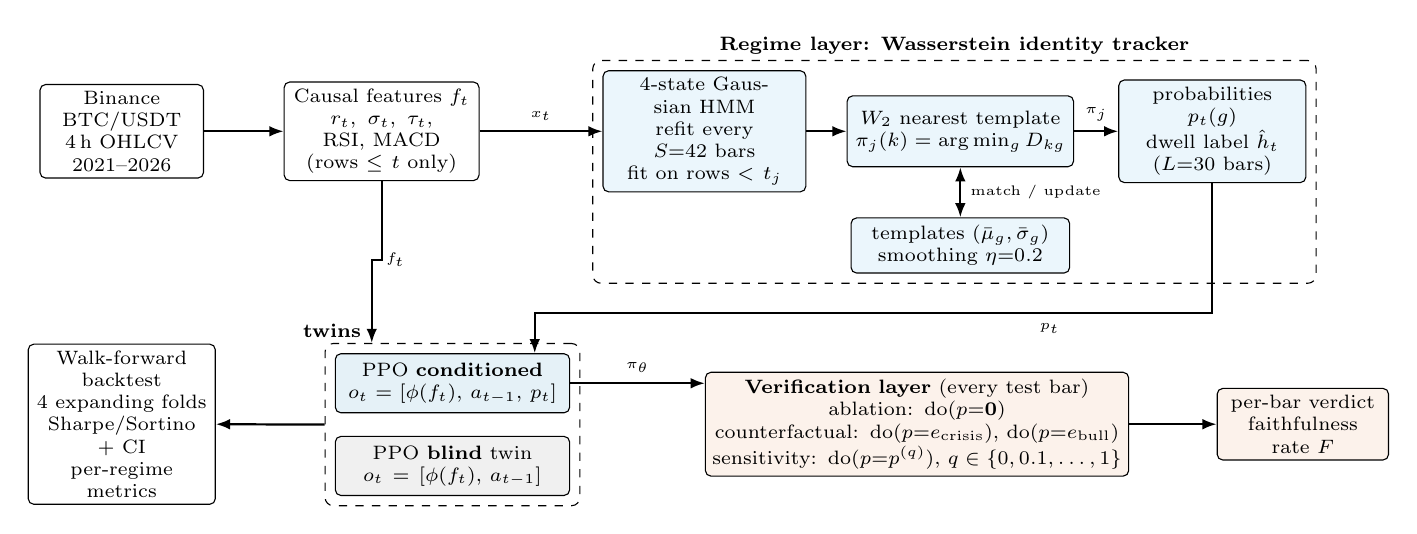
\begin{tikzpicture}[
  font=\scriptsize,
  box/.style={draw, rounded corners=2pt, align=center, minimum height=9mm, inner sep=2.5pt, fill=white},
  grp/.style={draw, dashed, rounded corners=3pt, inner sep=3.5pt},
  arr/.style={-{Latex[length=1.8mm]}, thick}]
% row 1: data and regime layer
\node[box, text width=19mm] (data) at (0,0) {Binance BTC/USDT\\4\,h OHLCV\\2021--2026};
\node[box, text width=23mm] (feat) at (3.3,0) {Causal features $f_t$\\$r_t,\ \sigma_t,\ \tau_t$, RSI, MACD\\(rows $\le t$ only)};
\node[box, text width=24mm, fill=ccalm!12] (hmm) at (7.4,0) {4-state Gaussian HMM\\refit every $S{=}42$ bars\\fit on rows $<t_j$};
\node[box, text width=27mm, fill=ccalm!12] (match) at (10.65,0) {$\Wtwo$ nearest template\\$\pi_j(k)=\arg\min_g D_{kg}$};
\node[box, text width=22mm, fill=ccalm!12] (agg) at (13.85,0) {probabilities $p_t(g)$\\dwell label $\hat h_t$\\($L{=}30$ bars)};
\node[box, text width=26mm, fill=ccalm!12, minimum height=7mm] (tmpl) at (10.65,-1.45) {templates $(\bar\mu_g,\bar\sigma_g)$\\smoothing $\eta{=}0.2$};
\begin{scope}[on background layer]
\node[grp, fit=(hmm)(match)(agg)(tmpl), label={[font=\scriptsize\bfseries, yshift=-0.5mm]above:Regime layer: Wasserstein identity tracker}] (rl) {};
\end{scope}
% row 2: agents, backtest, verification
\node[box, text width=28mm, fill=cblue!10, minimum height=7.5mm] (cond) at (4.2,-3.2) {PPO \textbf{conditioned}\\$o_t=[\phi(f_t),\,a_{t-1},\,p_t]$};
\node[box, text width=28mm, fill=gray!12, minimum height=7.5mm] (blind) at (4.2,-4.25) {PPO \textbf{blind} twin\\$o_t=[\phi(f_t),\,a_{t-1}]$};
\begin{scope}[on background layer]
\node[grp, fit=(cond)(blind), label={[font=\scriptsize\bfseries, yshift=-0.5mm]above left:twins}] (tw) {};
\end{scope}
\node[box, text width=22mm] (bt) at (0,-3.72) {Walk-forward backtest\\4 expanding folds\\Sharpe/Sortino + CI\\per-regime metrics};
\node[box, text width=52mm, fill=ccrisis!8] (ver) at (10.1,-3.72) {\textbf{Verification layer} (every test bar)\\
ablation: $\mathrm{do}(p{=}\mathbf 0)$\\
counterfactual: $\mathrm{do}(p{=}e_{\text{crisis}})$, $\mathrm{do}(p{=}e_{\text{bull}})$\\
sensitivity: $\mathrm{do}(p{=}p^{(q)})$, $q\in\{0,0.1,\dots,1\}$};
\node[box, text width=20mm, fill=ccrisis!8] (verdict) at (15.0,-3.72) {per-bar verdict\\faithfulness rate $F$};
% arrows
\draw[arr] (data) -- (feat);
\draw[arr] (feat) -- node[above, font=\tiny]{$x_t$} (hmm);
\draw[arr] (hmm) -- (match);
\draw[arr] (match) -- node[above, font=\tiny]{$\pi_j$} (agg);
\draw[{Latex[length=1.8mm]}-{Latex[length=1.8mm]}, thick] (tmpl) -- node[right, font=\tiny]{match / update} (match);
\draw[arr] (feat.south) -- ++(0,-1.0) -| node[pos=0.3, right, font=\tiny]{$f_t$} ($(tw.north west)+(0.6,0)$);
\draw[arr] (agg.south) -- ++(0,-1.65) -| node[pos=0.12, below, font=\tiny]{$p_t$} ($(cond.north east)+(-0.45,0)$);
\draw[arr] (tw.west) -- (bt.east);
\draw[arr] (cond.east) -- node[above, font=\tiny]{$\pi_\theta$} (cond.east -| ver.west);
\draw[arr] (ver) -- (verdict);
\end{tikzpicture}
\caption{System architecture. Features are causal. The regime layer refits the HMM on past rows only, names its components by Wasserstein distance to persistent templates, and passes the aggregated probabilities $p_t$ to the conditioned agent. The blind twin differs only in lacking $p_t$. Every out-of-fold decision of the conditioned agent is audited by three interventions on $p_t$.}
\label{fig:arch}
\end{figure*}

\subsection{Data and causal features}
Let $C_t$ be the close of bar $t$. The features are the log return $r_t=\log(C_t/C_{t-1})$, the 20-bar rolling standard deviation $\sigma_t$ of $r$, the trend $\tau_t=C_t/\mathrm{SMA}_{20}(C)_t-1$, the 14-bar Wilder RSI scaled to $[0,1]$, and the MACD histogram (EMA$_{12}-$EMA$_{26}$ minus its 9-bar signal) divided by $C_t$. Each feature at $t$ uses rows $\le t$ only. A unit test checks that features computed on a truncated history equal the prefix of the full computation. The regime model uses $x_t=(r_t,\sigma_t,\tau_t)$. The agent sees all five as $f_t$, rescaled to unit order by a fixed map $\phi$ ($r,\sigma,\text{MACD}\times100$; $\tau\times10$; RSI$\mapsto 2\,\text{RSI}-1$).

\subsection{Walk-forward HMM refits}
The tracker makes a single forward pass over the series (Fig.~\ref{fig:timeline}). The first $B=252$ bars (six weeks) form a burn-in. After that, refit $j$ starts at $t_j=B+jS$ with stride $S=42$ bars (one week). At each refit a four-state diagonal HMM is fitted by EM (200 iterations, seed 42) to the rows strictly before $t_j$, standardised with that window's mean $\bar x$ and standard deviation $s$. The model then decodes the window $W_j=\{t_j,\dots,t_j+S-1\}$. Component parameters are mapped back to feature units so that different fits can be compared:
\begin{equation}
\mu_k=\hat m_k\odot s+\bar x,\qquad \sigma_k=\sqrt{\hat v_k}\odot s .
\end{equation}

\begin{figure}[t]
\centering
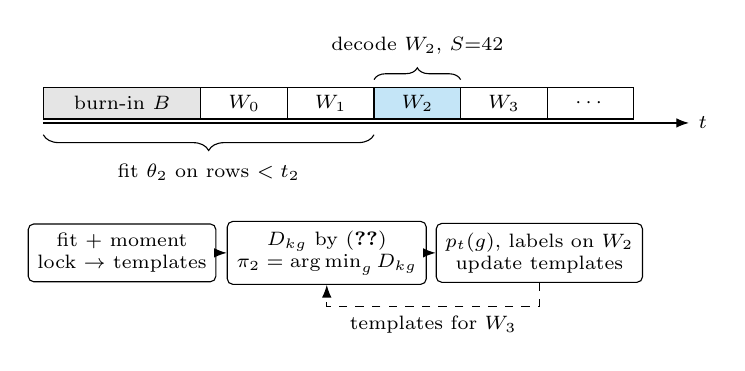
\begin{tikzpicture}[font=\scriptsize, x=1mm, y=1mm]
\fill[gray!20] (0,0) rectangle (20,4);
\node at (10,2) {burn-in $B$};
\foreach \i/\c in {0/white,1/white,2/ccalm!35,3/white,4/white} {
  \fill[\c] ({20+\i*11},0) rectangle ({31+\i*11},4);
  \draw ({20+\i*11},0) rectangle ({31+\i*11},4);
}
\draw (0,0) rectangle (20,4);
\node at (25.5,2) {$W_0$}; \node at (36.5,2) {$W_1$}; \node at (47.5,2) {$W_2$}; \node at (58.5,2) {$W_3$}; \node at (69.5,2) {$\cdots$};
\draw[-{Latex[length=1.6mm]}] (0,-0.5) -- (82,-0.5) node[right]{$t$};
\draw[decorate, decoration={brace, amplitude=2mm, mirror}] (0,-2) -- (42,-2) node[midway, below=2.5mm, align=center] {fit $\theta_2$ on rows $<t_2$};
\draw[decorate, decoration={brace, amplitude=1.5mm}] (42,5) -- (53,5) node[midway, above=2mm] {decode $W_2$, $S{=}42$};
\node[draw, rounded corners=2pt, align=center, fill=white] (a) at (10,-17) {fit + moment\\lock $\to$ templates};
\node[draw, rounded corners=2pt, align=center, fill=white] (b) at (36,-17) {$D_{kg}$ by \eqref{eq:w2diag}\\$\pi_2=\argmin_g D_{kg}$};
\node[draw, rounded corners=2pt, align=center, fill=white] (c) at (63,-17) {$p_t(g)$, labels on $W_2$\\update templates};
\draw[-{Latex[length=1.6mm]}] (a) -- (b);
\draw[-{Latex[length=1.6mm]}] (b) -- (c);
\draw[-{Latex[length=1.6mm]}, dashed] (c.south) -- ++(0,-3) -| node[pos=0.25, below]{templates for $W_3$} (b.south);
\end{tikzpicture}
\caption{Causal refit schedule. The burn-in fit names the templates once by moment sorting. Every later window is decoded by a model fitted only on earlier rows, and its components inherit names by Wasserstein matching. Labels already issued are never revised.}
\label{fig:timeline}
\end{figure}

\subsection{Template initialisation}
The burn-in fit is the only place where names come from moments. The rule $\ell$ sorts components by mean return. Of the two lowest, the one with lower volatility is \emph{bear} and the other is \emph{crisis}. Of the two highest, the one with lower volatility is \emph{calm} and the other is \emph{bull}. This yields templates $(\bar\mu_g,\bar\sigma_g)$ for $g\in\G=\{\text{bull},\text{bear},\text{calm},\text{crisis}\}$.

\subsection{Wasserstein identity matching}
At refit $j$ the cost of naming component $k$ as regime $g$ is the diagonal Wasserstein distance~\eqref{eq:w2diag}:
\begin{equation}
D_{kg}=\lVert\mu_k-\bar\mu_g\rVert^2+\lVert\sigma_k-\bar\sigma_g\rVert^2 ,
\end{equation}
and every component takes its nearest template independently,
\begin{equation}
\pi_j(k)=\argmin_{g\in\G} D_{kg}.
\label{eq:match}
\end{equation}
The matching need not be one-to-one: two components may share a template, and a template may receive none. The regime probabilities for $t\in W_j$ are the summed posteriors
\begin{equation}
p_t(g)=\sum_{k:\,\pi_j(k)=g}\gamma_t(k),
\label{eq:agg}
\end{equation}
and an unmatched template has $p_t(g)=0$.

\subsection{Template smoothing}
After window $W_j$ is labelled, every matched template moves a step $\eta=0.2$ toward its members. Let $w_k=\sum_{t\in W_j}\gamma_t(k)$ and $\omega_k=w_k/\sum_{k'\in M_g}w_{k'}$ for the member set $M_g=\{k:\pi_j(k)=g\}$. Then
\begin{equation}
\bar\mu_g\leftarrow(1-\eta)\,\bar\mu_g+\eta\sum_{k\in M_g}\omega_k\mu_k ,
\label{eq:update}
\end{equation}
and likewise for $\bar\sigma_g$. A template with $M_g=\emptyset$ is left unchanged. The update uses window $W_j$ and affects only windows after it.

\subsection{Hard labels and dwell constraint}
The hard label $\hat h_t$ is the name of the Viterbi state, $\pi_j(\hat z_t)$. Runs shorter than $L=30$ bars (five days) are merged into the preceding label, with the last issued label carried across window boundaries. Hard labels are used only for reporting and per-regime evaluation. The agent sees the probabilities $p_t$.

\subsection{Twin agents}
\label{sec:twins}
The trading environment is a Gymnasium episode over the training rows. At bar $t$ the agent chooses a target position $a_t\in[-1,1]$ and receives
\begin{equation}
R_t=a_t\,r_{t+1}-c\,\lvert a_t-a_{t-1}\rvert,\qquad c=10^{-3},
\label{eq:reward}
\end{equation}
that is, the next log return less a 10-basis-point turnover cost. The conditioned agent observes $o_t=[\phi(f_t),a_{t-1},p_t]\in\R^{10}$ and the blind twin observes $[\phi(f_t),a_{t-1}]\in\R^{6}$. Both are PPO agents from Stable-Baselines3 with identical settings (Table~\ref{tab:hyper}). The only architectural difference is four extra input weights in the first layer, and that difference is the experiment.

\subsection{Verification suite}
For each out-of-fold bar we freeze the conditioned policy, the market features and the previous position, and intervene on $p$ alone. Let $a_t=\pi_\theta(u_t,p_t)$ be the realised action, $e_g$ the one-hot vector of regime $g$, and $\rho$ a defensive rank with $\rho(\text{bull})=0<\rho(\text{calm})=1<\rho(\text{bear})=2<\rho(\text{crisis})=3$.

\emph{Ablation.} The regime input is load-bearing at $t$ if
\begin{equation}
\Delta^{\text{ab}}_t=\bigl\lvert a_t-\pi_\theta(u_t,\mathrm{do}(p{=}\mathbf 0))\bigr\rvert\ \ge\ \delta_{\text{ab}}=0.15 .
\end{equation}

\emph{Counterfactual.} With $g_t=\argmax_g p_t(g)$, forcing crisis must cut the position and forcing bull must raise it, each by at least $\delta_{\text{cf}}=0.10$, whenever the forced regime differs in rank from $g_t$:
\begin{align}
\rho(g_t)<3 &\Rightarrow a_t-\pi_\theta(u_t,\mathrm{do}(p{=}e_{\text{crisis}}))\ge\delta_{\text{cf}},\\
\rho(g_t)>0 &\Rightarrow \pi_\theta(u_t,\mathrm{do}(p{=}e_{\text{bull}}))-a_t\ge\delta_{\text{cf}}.
\end{align}

\emph{Sensitivity.} For $q\in\{0,0.1,\dots,1\}$ we inject a crisis probability $q$ and rescale the other entries:
\begin{equation}
p^{(q)}=(1-q)\,\frac{p_t^{\setminus c}}{\lVert p_t^{\setminus c}\rVert_1}+q\,e_{\text{crisis}},
\end{equation}
where $p_t^{\setminus c}$ is $p_t$ with its crisis entry set to zero (uniform over the other three if that leaves nothing). The curve $y_i=\pi_\theta(u_t,\mathrm{do}(p{=}p^{(q_i)}))$ passes if it rises at most once, $\sum_i\mathbb 1[y_{i+1}>y_i+10^{-8}]\le 1$.

A bar is \emph{faithful} when all three checks pass. The faithfulness rate $F$ is the share of faithful bars. Each bar costs 15 batched forward passes.

%======================================================================
\section{Experimental Setup}
%======================================================================
\subsection{Data and folds}
We use Binance BTC/USDT four-hour candles from 1~Jan 2021 to 22~Sep 2026 (12{,}544 bars). Feature warm-up leaves 12{,}510 bars. Four expanding walk-forward folds start with 1{,}080 training bars, and each test block has about 2{,}857 bars (Table~\ref{tab:folds}). Each test block is scored by agents trained only on the bars before it. The concatenated test blocks give 11{,}430 out-of-fold bars from 5~Jul 2021 to 22~Sep 2026. Regime labels for every bar come from the single causal tracker pass described above.

\begin{table}[t]
\caption{Walk-forward folds and per-fold Sharpe ratios (annualised, out of fold)}
\label{tab:folds}
\centering
\setlength{\tabcolsep}{3.2pt}
\begin{tabular}{@{}clrrrrr@{}}
\toprule
Fold & Test period & Train & Cond. & Blind & B\&H & Cond.$^\dagger$\\
\midrule
0 & 07/2021--10/2022 & 1{,}080 & $-1.95$ & $-1.84$ & $-0.65$ & $-2.32$\\
1 & 10/2022--02/2024 & 3{,}937 & $0.24$ & $-3.29$ & $1.69$ & $-0.53$\\
2 & 02/2024--06/2025 & 6{,}794 & $0.53$ & $0.66$ & $1.10$ & $2.24$\\
3 & 06/2025--09/2026 & 9{,}651 & $0.50$ & $-0.79$ & $-0.39$ & $1.93$\\
\bottomrule
\multicolumn{7}{@{}l@{}}{\footnotesize $^\dagger$Archived run with per-fold moment-sorted labels (see Sec.~\ref{sec:baselines}).}
\end{tabular}
\end{table}

\subsection{Implementation details}
Table~\ref{tab:hyper} lists the settings. PPO uses the Stable-Baselines3 defaults for clipping (0.2) and epochs per update (10). Each agent trains for $\max(8192, 10\,N_{\text{train}})$ steps, which is ten passes over its training window: 10{,}800, 39{,}370, 67{,}940 and 96{,}510 steps for the four folds. HMMs are fitted with \texttt{hmmlearn}. If EM leaves a state with an all-zero transition row, that row is reset to uniform before decoding. The full pipeline (292 tracker refits, eight PPO trainings and the audit) ran in 6.6 minutes on a laptop CPU. All 25 unit tests of the repository pass, including tests for feature leakage, the closed-form distance, label stability under a component swap, and that later bars never change a closed window.

\begin{table}[t]
\caption{Implementation settings (from the project code)}
\label{tab:hyper}
\centering
\setlength{\tabcolsep}{4pt}
\begin{tabular}{@{}ll@{}}
\toprule
Component & Setting\\
\midrule
HMM & 4 states, diagonal cov., EM 200 it., min. cov. $10^{-3}$\\
Tracker & burn-in $B{=}252$, stride $S{=}42$, $\eta{=}0.2$, dwell $L{=}30$\\
Policy net & MLP $64{-}64$, $\tanh$, Gaussian action head\\
PPO & lr $3{\times}10^{-4}$, $\gamma{=}0.99$, $\lambda_{\text{GAE}}{=}0.95$, entropy 0\\
Rollout & $n_{\text{steps}}{=}256$, batch 64, seed 42, CPU\\
Cost & $c=10^{-3}$ per unit turnover\\
Verifier & $\delta_{\text{ab}}{=}0.15$, $\delta_{\text{cf}}{=}0.10$, 11-point sweep, $\le$1 uptick\\
Bootstrap & 1{,}000 i.i.d. resamples, 95\% percentile CI\\
\bottomrule
\end{tabular}
\end{table}

\subsection{Baselines}
\label{sec:baselines}
\emph{Blind twin.} The same PPO agent without $p_t$ (Sec.~\ref{sec:twins}).
\emph{Buy-and-hold.} A constant position $a_t=1$.
\emph{Archived moment-sort run.} The repository keeps the outputs of the pipeline as it stood before the tracker was introduced. That version fitted one HMM per fold and named states with $\ell$ alone, and everything else was identical. Its blind-twin and buy-and-hold results match ours exactly, so the labels are the only change.
\emph{Moment sorting on the same refits.} To isolate the identity rule, we also re-name every one of the 292 refits with $\ell$ instead of~\eqref{eq:match}. This variant is used for label statistics only.
\emph{Reference policies for the verifier.} The rule $a=\mathrm{clip}(p^\top w)$ with $w=(1,-0.4,0.5,-1)$ over (bull, bear, calm, crisis) is faithful by construction. A constant $a=0.5$ ignores the regime input, and $a=\mathrm{clip}(-p^\top w)$ inverts it.

\subsection{Metrics}
Strategy log returns follow~\eqref{eq:reward} with the realised positions. We report the annualised Sharpe ratio $\sqrt{2190}\,\bar R/\hat s_R$ and the Sortino ratio $\sqrt{2190}\,\bar R/\sqrt{\overline{\min(R,0)^2}}$, using 2{,}190 four-hour bars per year. Each comes with a 95\% bootstrap interval. We also report maximum drawdown and total return. Every metric is additionally computed within each dwell-smoothed regime. For the tracker we report label shares, switches per year, run lengths, the mean matched $\Wtwo^2$ cost, and an identity-jump statistic: the $\Wtwo^2$ distance between the probability-weighted components that carry the same name at consecutive refits.

%======================================================================
\section{Results and Discussion}
%======================================================================
\subsection{Regime identity under refits}
\label{sec:identity}
Fig.~\ref{fig:regimes} shows the price with the tracker's labels, the bear and crisis probabilities, and both labellings. Table~\ref{tab:labels} compares them. Moment sorting assigns a different name than the $\Wtwo$ rule to at least one component in 291 of the 292 refits, and to 49.6\% of all components. Its labels are semantically unstable. Over the sample, the bars it calls \emph{bull} have a negative mean return ($-0.8$\,bp), and its \emph{crisis} bars are only slightly more volatile than its \emph{calm} bars (1.14\% against 1.04\%). The $\Wtwo$ tracker keeps the ordering the names promise: crisis bars average 2.18\% volatility and $-8.1$\,bp per bar, against 0.97\% and $+1.5$\,bp for calm. It also switches less often (5.5 against 7.5 times per year). Its matched cost is 4.9 times lower ($1.88$ against $9.13\times10^{-4}$), and the identity jump of the crisis name falls by a factor of 7.4.

\begin{figure*}[t]
\centering
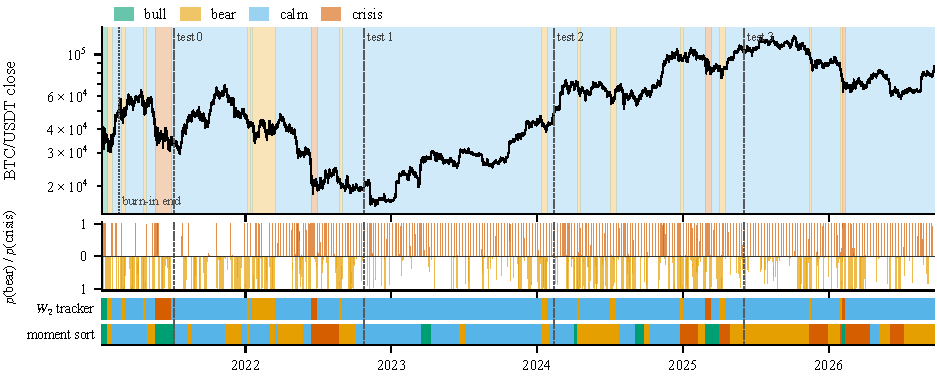
\includegraphics[width=\textwidth]{figures/regime_price.pdf}
\caption{BTC/USDT four-hour close (log scale) shaded by the dwell-smoothed $\Wtwo$ tracker label (top). Tracker probabilities of crisis (up) and bear (down) (middle). Labels from the $\Wtwo$ tracker and from moment sorting on the same 292 refits (bottom). Dashed lines mark the start of each test fold.}
\label{fig:regimes}
\end{figure*}

\begin{table}[t]
\caption{Regime labels after burn-in (12{,}258 bars): share of bars, mean 4\,h log return and mean $\sigma_{20}$ per label}
\label{tab:labels}
\centering
\setlength{\tabcolsep}{2.6pt}
\begin{tabular}{@{}l rrr rrr@{}}
\toprule
 & \multicolumn{3}{c}{$\Wtwo$ tracker (ours)} & \multicolumn{3}{c}{Moment sort per refit}\\
\cmidrule(lr){2-4}\cmidrule(l){5-7}
Label & share & ret (bp) & $\sigma$ (\%) & share & ret (bp) & $\sigma$ (\%)\\
\midrule
bull   & 0.0\% & --       & --   & 7.2\%  & $-0.8$ & 1.54\\
bear   & 7.7\% & $-7.7$   & 1.42 & 34.2\% & $-3.1$ & 0.93\\
calm   & 88.5\% & $+1.5$  & 0.97 & 44.2\% & $+3.7$ & 1.04\\
crisis & 3.8\% & $-8.1$   & 2.18 & 14.4\% & $-0.6$ & 1.14\\
\midrule
switches / yr & \multicolumn{3}{c}{5.5} & \multicolumn{3}{c}{7.5}\\
median run (bars) & \multicolumn{3}{c}{110} & \multicolumn{3}{c}{210}\\
mean matched $\Wtwo^2$ ($10^{-4}$) & \multicolumn{3}{c}{1.88} & \multicolumn{3}{c}{9.13}\\
\bottomrule
\end{tabular}
\end{table}

These gains have a price. Matching~\eqref{eq:match} is non-injective in 291 of the 292 refits. Fig.~\ref{fig:templates} shows why. The bull template inherits the burn-in's high-volatility, high-return component from early 2021. Later fits never produce a component near it, so it receives members in only 35 refits. Under~\eqref{eq:update} an unmatched template never moves, so after mid-2022 the bull template stays frozen. Calm absorbs the slack and covers 88.5\% of bars, and no bar is labelled bull after burn-in. Fig.~\ref{fig:w2} shows a refit during the June 2022 crash. Components 0 and 2 both map to calm, while moment sorting would have called component~0 bull. A diagnostic variant (not part of the pipeline) replaces~\eqref{eq:match} with a one-to-one Hungarian assignment. It brings bull back to 5.1\% of bars, with a mean return of $+11.9$\,bp, but crisis then grows to 31.3\% and its volatility falls to 1.15\%. Neither rule alone keeps both coverage and sharp semantics.

\begin{figure}[t]
\centering
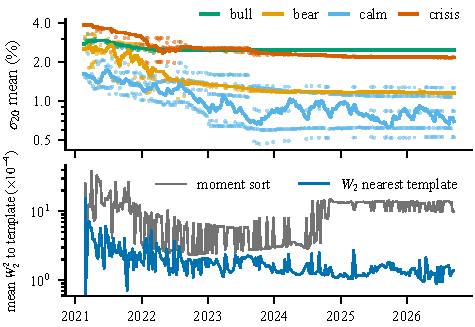
\includegraphics[width=\columnwidth]{figures/templates.pdf}
\caption{Top: template volatility (lines) and fitted component volatilities coloured by their $\Wtwo$ assignment (dots) at each refit. The bull template freezes once it stops receiving members. Bottom: mean squared $\Wtwo$ distance between components and the template they are named after, for the $\Wtwo$ rule and for moment sorting.}
\label{fig:templates}
\end{figure}

\begin{figure}[t]
\centering
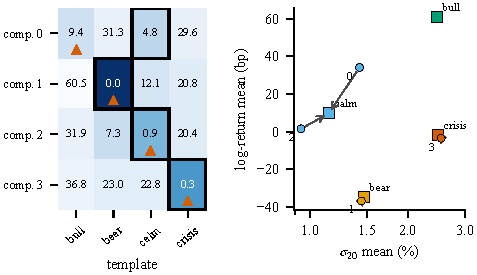
\includegraphics[width=\columnwidth]{figures/w2_matrix.pdf}
\caption{Refit of 15 Jun 2022. Left: $\Wtwo^2$ cost $D_{kg}$ ($\times10^{-4}$). Boxes mark the $\Wtwo$ assignment and triangles the moment-sort assignment. Right: components (circles) and templates (squares) in mean-volatility and mean-return space, with arrows to the assigned template.}
\label{fig:w2}
\end{figure}

\subsection{Trading performance}
Table~\ref{tab:perf} and Fig.~\ref{fig:equity} summarise performance out of fold. With $\Wtwo$ labels the conditioned agent has a Sharpe ratio of $-0.16$ and loses 29\% over the test period. Its blind twin does much worse ($-1.12$, $-93$\%), and buy-and-hold gains 156\% with a Sharpe of $0.35$. All bootstrap intervals for the conditioned agent overlap buy-and-hold, and only the blind twin's interval excludes zero. The archived run with moment-sorted labels reached $0.41$, mostly through folds 2 and 3 (Table~\ref{tab:folds}). Its interval overlaps ours, so the regime-layer change cannot be said to have hurt returns significantly.

\begin{table}[t]
\caption{Out-of-fold performance, 11{,}430 bars (95\% bootstrap CI)}
\label{tab:perf}
\centering
\setlength{\tabcolsep}{3.5pt}
\renewcommand{\arraystretch}{1.05}
\begin{tabular}{@{}lccrr@{}}
\toprule
System & Sharpe & Sortino & MDD & Return\\
\midrule
Conditioned ($\Wtwo$) & \ci{-0.16}{-0.98}{0.63} & \ci{-0.22}{-1.34}{0.91} & $-77.0\%$ & $-29.3\%$\\
Blind twin & \ci{-1.12}{-1.96}{-0.27} & \ci{-1.51}{-2.55}{-0.37} & $-94.4\%$ & $-93.0\%$\\
Buy-and-hold & \ci{0.35}{-0.51}{1.24} & \ci{0.50}{-0.71}{1.81} & $-77.0\%$ & $+156.2\%$\\
\midrule
Cond. (archived) & \ci{0.41}{-0.41}{1.20} & \ci{0.58}{-0.58}{1.77} & $-79.8\%$ & $+139.2\%$\\
\bottomrule
\end{tabular}
\end{table}

\begin{figure}[t]
\centering
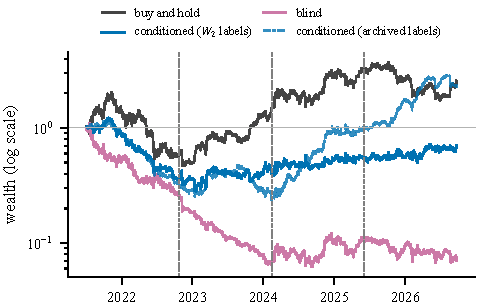
\includegraphics[width=\columnwidth]{figures/equity.pdf}
\caption{Out-of-fold wealth (log scale). Dashed vertical lines separate test folds. The dashed blue curve is the archived conditioned agent trained on moment-sorted labels.}
\label{fig:equity}
\end{figure}

The per-regime view (Table~\ref{tab:regime}) shows where the gap comes from. In bear and crisis segments the conditioned agent holds a net short position on average ($-0.23$ and $-0.17$), while the blind twin stays long ($+0.17$ and $+0.24$). Its Sharpe ratio in bear segments, $-0.19$, is far better than the blind twin's $-3.20$ and buy-and-hold's $-1.94$. In calm segments it is long but trails buy-and-hold. Crisis segments cover only 214 test bars, about five weeks, so their annualised ratios are very noisy. This is consistent with an agent that uses its regime input, at least for regimes it saw in training.

\begin{table}[t]
\caption{Per-regime Sharpe ratio and mean position (out of fold, $\Wtwo$ labels; no bar is labelled bull)}
\label{tab:regime}
\centering
\setlength{\tabcolsep}{3pt}
\begin{tabular}{@{}lrrrrrr@{}}
\toprule
 & & \multicolumn{3}{c}{Sharpe} & \multicolumn{2}{c}{mean position}\\
\cmidrule(lr){3-5}\cmidrule(l){6-7}
Regime & $n$ & Cond. & Blind & B\&H & Cond. & Blind\\
\midrule
bear   & 852    & $-0.19$ & $-3.20$ & $-1.94$ & $-0.23$ & $+0.17$\\
calm   & 10{,}364 & $-0.17$ & $-1.01$ & $0.71$ & $+0.41$ & $+0.25$\\
crisis & 214    & $0.19$  & $1.22$  & $-2.23$ & $-0.17$ & $+0.24$\\
\bottomrule
\end{tabular}
\end{table}

\subsection{Faithfulness}
Fig.~\ref{fig:faith} reports the pass rate of each check. The reference policies behave as designed. The faithful rule passes on 97.9\% of bars; it fails ablation only where its output is already within 0.15 of zero. The ignoring and inverted rules pass on no bar.

\begin{figure}[t]
\centering
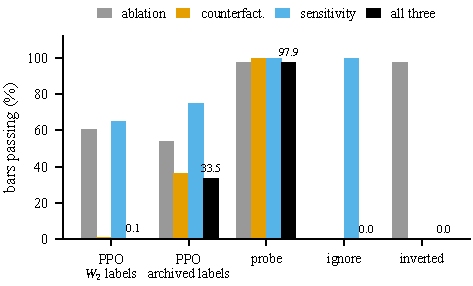
\includegraphics[width=\columnwidth]{figures/faithfulness.pdf}
\caption{Share of out-of-fold bars passing each check, for the PPO agent trained on $\Wtwo$ labels, the archived PPO agent trained on moment-sorted labels, and three reference policies scored on the $\Wtwo$ probabilities. Numbers give the share passing all three checks.}
\label{fig:faith}
\end{figure}

For the conditioned PPO agent with $\Wtwo$ labels, ablation passes on 60.7\% of bars, with a median $\lvert\Delta^{\text{ab}}\rvert$ of 0.42, so the regime input is clearly load-bearing. The counterfactual check, however, passes on only 0.9\% of bars, and the combined faithfulness rate is 0.1\% (11 of 11{,}430 bars). The archived agent reached 33.5\%. Fig.~\ref{fig:interv} explains the failure. Forcing \emph{bear} sends the median position to $-1$, and the forced-bear position lies below the forced-calm position on 76.5\% of bars. The agent has learned a defensive response, but it is keyed to bear. Forcing \emph{crisis} gives a median of $+0.64$, which is defensive relative to calm on only 30.1\% of bars. Forcing \emph{bull} gives $+0.53$, below the realised median of $+0.74$. Taken separately, the two directions of the counterfactual check pass on 23.3\% (crisis cuts the position) and 19.9\% (bull raises it) of eligible bars, and their conjunction almost never holds. The crisis sweep in Fig.~\ref{fig:interv}(a) tells the same story. For bear and crisis bars the mean position \emph{rises} as crisis probability is injected.

\begin{figure}[t]
\centering
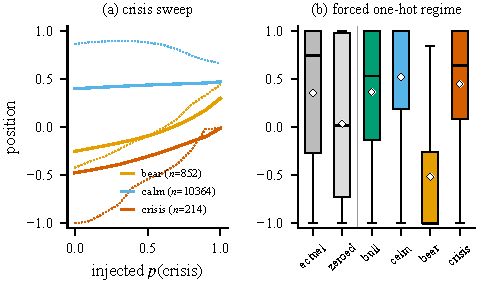
\includegraphics[width=\columnwidth]{figures/interventions.pdf}
\caption{Interventions on the conditioned agent ($\Wtwo$ labels). (a) Mean (solid) and median (dotted) position against injected crisis probability, grouped by the bar's label. (b) Distribution of the realised position, the position with the regime input zeroed, and positions under one-hot regime inputs (boxes: interquartile range; diamonds: means).}
\label{fig:interv}
\end{figure}

This behaviour follows from the regime layer. The tracker's probabilities are almost one-hot (mean maximum 0.975), and crisis occupies only 3.8\% of bars. One-hot bull never occurs in training after burn-in. The counterfactual inputs $e_{\text{bull}}$ and $e_{\text{crisis}}$ therefore lie far from, or entirely outside, the data the policy was fitted on. What the agent does there is an extrapolation, so the check fails without the agent being ``miswired'' on the inputs it actually meets. The archived labels kept all four regimes populated (bull 6.1\%, crisis 12.4\% of test bars), and their counterfactuals were in distribution. That, more than any quality of the agent, explains the archived 33.5\%. Two further caveats concern the checks themselves. The counterfactual rank uses $\argmax_g p_t(g)$, which agrees with the dwell-smoothed label on only 78.8\% of bars. And the sensitivity check is weak, since a flat curve passes it. On 18~Jun~2022, near the crash low, $p_t(\text{crisis})=1$ and the agent is fully long. Every intervention returns $+1$, so ablation and counterfactual fail while sensitivity passes. The ignoring policy passes sensitivity on every bar for the same reason.

The lesson is methodological. Swapping one well-motivated regime component for another, with architecture, data and training unchanged, improved label semantics and reversed the faithfulness verdict. A verdict cannot be carried over to a modified pipeline.

%======================================================================
\section{Limitations and Future Work}
%======================================================================
\emph{Within-window smoothing.} Each HMM is fitted only on rows before its window, but decoding uses Viterbi and forward--backward over the whole 42-bar window. The probability at a bar therefore conditions on up to 41 later bars of the same window, and the dwell merge similarly needs a run to finish before it can be judged. Labels are never revised after their window closes, but they are not strictly filtered. A forward-only (filtered) posterior and an online dwell rule would remove this leakage. Until then, the per-regime results should be read with this caveat.

\emph{Template starvation.} Non-injective matching with a frozen unmatched template removes the bull regime. One-to-one matching is not a complete fix either (Sec.~\ref{sec:identity}). Template birth and death, and a longer or multi-cycle burn-in, are natural next steps.

\emph{Counterfactual design.} One-hot interventions test the policy off its training distribution. Drawing counterfactual regime vectors from the empirical distribution of $p_t$, and adding a sensitivity criterion that requires a minimum range, would make the verdict more informative.

\emph{Statistics.} The i.i.d. bootstrap ignores the serial dependence of four-hour returns. A stationary block bootstrap would give wider and more honest intervals. All results come from a single PPO seed and a single asset.

\emph{Scope.} The thresholds $\delta_{\text{ab}}$ and $\delta_{\text{cf}}$ and the defensive ordering $\rho$ are design choices. Transaction costs are a flat 10\,bp, and the agents were built directly on Stable-Baselines3. Ndoutoumou \emph{et al.} instead place the regime signal inside the FinRL stack~\cite{ndoutoumou2025hmm}.

%======================================================================
\section{Conclusion}
%======================================================================
We built a regime-conditioned RL trading agent with a Wasserstein identity tracker and a suite that intervenes on the regime input of every decision. On five years of BTC/USDT four-hour data, the tracker produced labels whose meaning stayed stable across 292 causal refits, which moment sorting did not. The conditioned agent used those labels: removing them changed its position on most bars, and it reduced exposure in bear and crisis segments, where its blind twin did not. Yet it almost never responded to injected regimes in the direction their names imply, because template starvation left the injected states outside its training data. With the same agent and data, an earlier labelling gave a faithfulness rate of 33.5\%; with the new one the rate is 0.1\%. Regime-aware agents should report a faithfulness verdict next to their returns and recompute it whenever an upstream component changes; the suite here is cheap enough to do so routinely.

\bibliographystyle{IEEEtran}
\bibliography{references}

\end{document}
